\begin{tasks}
    \task 只有(1) \tab (1) only
    \task 只有(2) \tab (2) only
    \task 只有(3) \tab (3) only
    \task 只有(1)和(2) \tab (1) and (2) only
    \task 只有(1)和(3) \tab (1) and (3) only
    \task 只有(2)和(3) \tab (2) and (3) only
    \task (1), (2) 和 (3)\tab (1), (2) and (3)
\end{tasks}

\begin{tasks}
    \task 只有(1)
    \task 只有(2)
    \task 只有(3)
    \task 只有(1)和(2)
    \task 只有(1)和(3)
    \task 只有(2)和(3)
    \task (1), (2) 和 (3)
\end{tasks}

\begin{tasks}
    \task 只有(1) \tab\tab (1) only
    \task 只有(2) \tab\tab (2) only
    \task 只有(3) \tab\tab (3) only
    \task 只有(1)和(2) \tab\tab (1) and (2) only
    \task 只有(1)和(3) \tab\tab (1) and (3) only
    \task 只有(2)和(3) \tab\tab (2) and (3) only
    \task (1), (2) 和 (3)\tab\tab (1), (2) and (3)
\end{tasks}

\begin{tasks} [before-skip=0em,after-item-skip=0em]
    \task 只有(1) \tab (1) only
    \task 只有(2) \tab (2) only
    \task 只有(3) \tab (3) only
    \task 只有(1)和(2) \tab (1) and (2) only
    \task 只有(1)和(3) \tab (1) and (3) only
    \task 只有(2)和(3) \tab (2) and (3) only
    \task (1), (2) 和 (3)\tab (1), (2) and (3)
\end{tasks}

\begin{tasks}[item-indent=2em,label-offset=0em,before-skip=0em,after-item-skip=.8em](2)
    \task [] \textbf{透鏡類型lens}
    \task [] \textbf{影像的大小變化\\change in size of image}
    \task [] \rule{1.5in}{.5pt}
    \task [] \rule{1.5in}{.5pt}

\end{tasks}

\begin{choices}
    \choice 只有(1)和(2) \tab (1) and (2) only
    \choice 只有(1)和(3) \tab (1) and (3) only
    \choice 只有(2)和(3) \tab (2) and (3) only
    \choice (1), (2) 和 (3)\tab (1), (2) and (3)
\end{choices}
\begin{choices}
    \choice 只有(1)和(2) \tab (1) and (2) only
    \choice 只有(1)和(3) \tab (1) and (3) only
    \choice 只有(2)和(3) \tab (2) and (3) only
    \choice (1), (2) 和 (3)\tab (1), (2) and (3)
\end{choices}


\question\vspace{1cm}
\begin{samepage}
    \begin{enumerate}[label=\sd]
        \item
              \par
        \item
              \par
        \item
              \par
    \end{enumerate}
\end{samepage}
\begin{samepage}
    \begin{choices}
        \choice 只有(1)和(2) \tab (1) and (2) only
        \choice 只有(1)和(3) \tab (1) and (3) only
        \choice 只有(2)和(3) \tab (2) and (3) only
        \choice (1), (2) 和 (3)\tab (1), (2) and (3)
    \end{choices}
\end{samepage}

\question\vspace{1cm}
\begin{schoices}
    \choice
    \choice
    \choice
\end{schoices}
\begin{mchoices}
    \choice
    \choice
    \choice
    \item
\end{mchoices}

\question\vspace{1cm}
\begin{samepage}
    \begin{enumerate}[label=\sd]
        \item
              \par
        \item
              \par
        \item
              \par
    \end{enumerate}
\end{samepage}
\begin{samepage}
    \begin{choices}
        \choice 只有(1)
        \choice 只有(2)
        \choice 只有(1)和(3)
        \choice 只有(2)和(3)
    \end{choices}
\end{samepage}

% main
\begin{samepage}
    \question\vspace{1cm}

    \begin{choices}
        \choice
        \choice
        \choice
        \choice
    \end{choices}
\end{samepage}



\question\vspace{1cm}
\begin{samepage}
    \par\hspace{4.5em}$R_2$\hspace{7em} $R_3$
    \begin{choices}
        \choice
        \choice
        \choice
        \choice
    \end{choices}
\end{samepage}

\question
\begin{choices}
    \begin{multicols}{2}
        \choice
        \adjustbox{valign=t}{\includegraphics[scale=0.2]{example-image-a}}
        \choice
        \adjustbox{valign=t}{\includegraphics[scale=0.2]{example-image-b}}
    \end{multicols}\par
    \begin{multicols}{2}
        \choice
        \adjustbox{valign=t}{\includegraphics[scale=0.2]{example-image-c}}
        \CorrectChoice
        \adjustbox{valign=t}{\includegraphics[scale=0.2]{example-image-a}}
    \end{multicols}
\end{choices}

\question
\adjustbox{valign=t}{\includegraphics[width=0.7\linewidth]{images/Screenshot 2023-09-12 at 6.40.46 AM.png}}


\begin{mmchoices}
    \item \topalign{
        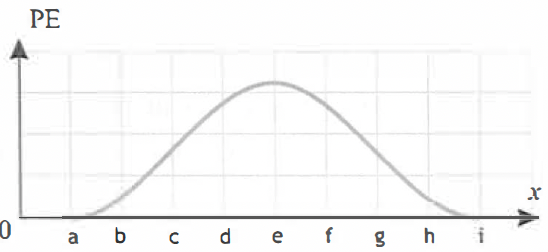
\includegraphics[width=0.75\linewidth]{images/Screenshot 2023-09-27 at 8.30.49 AM.png}
    }
    \item \topalign{
        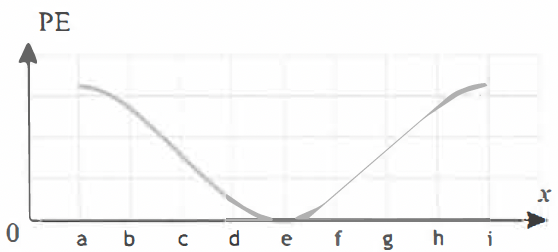
\includegraphics[width=0.75\linewidth]{images/Screenshot 2023-09-27 at 8.30.55 AM.png}
    }
    \item \topalign{
        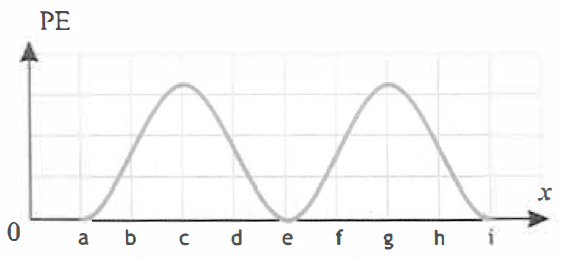
\includegraphics[width=0.75\linewidth]{Screenshot 2023-09-27 at 8.31.00 AM.png}
    }
    \item \topalign{
        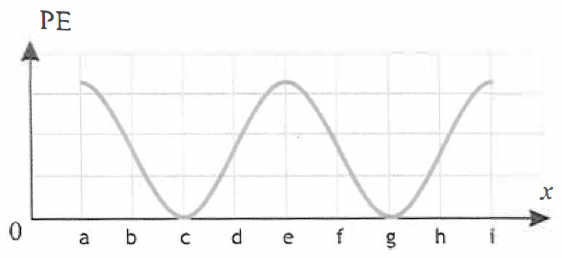
\includegraphics[width=0.75\linewidth]{images/Screenshot 2023-09-27 at 8.31.03 AM.png}
    }
\end{mmchoices}


\begin{statements}
    [before-skip=0pt,after-item-skip=0pt,label-offset=1em,item-indent=2em] (2)
    \task
    \topalign{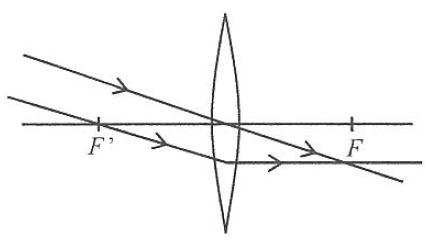
\includegraphics[width=.9\linewidth]{assets/x1nue9812.png}}


    \task
    \topalign{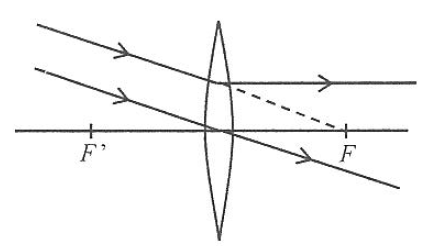
\includegraphics[width=.9\linewidth]{assets/xn1e891age.png}}

    \task
    \topalign{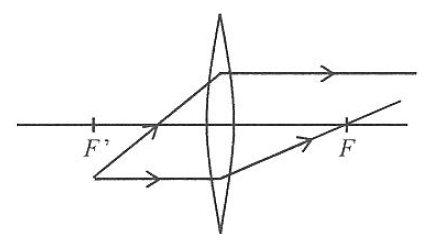
\includegraphics[width=.9\linewidth]{assets/x8n9u009e03298enx923.png}}



\end{statements}